\section{Localisation en intérieur}
\label{sec:localisation}

Le plus grand défi de ce projet est la localisation en intérieur de l'utilisateur, par là, le degré de précision de cette localisation. De plus, il est intéressant et agréable pour l'utilisateur de disposer d'un suivi régulier de sa position durant la visualisation 3D. Cette section explique les diverses pistes empruntées ainsi que leurs résultats.

\subsection{GPS}
Qui dit localisation pense GPS (\textit{Global Positioning System}), système qui pourrait, à première vue, présenter une bonne solution. Cependant, cette technologie manque de précision, principalement en intérieur. La précision des GPS mobiles se situerait à peu près entre 4 et 50 mètres, dépendant des conditions et du smartphone utilisé. En général, l'erreur est due aux éléments entre l'utilisateur et le satellite, c'est pourquoi la localisation en intérieur ne peut pas se fier au GPS.

\subsection{Triangulation Wifi}
Une méthode utilisée pour la localisation en intérieur est la triangulation / trilatération, en utilisant les \textit{Access Points} WiFi. Le concept consiste à retenir à l'avance les coordonnées de tous les AP. Chaque AP possède une adresse MAC qui les différencie les uns des autres. Ensuite, il faut scanner les AP depuis l'objet que l'ont veut localiser et, en fonction des forces des AP, il est possible de retrouver la position.

L'avantage de cette solution est l'absence d'infrastructures à mettre en place, étant donné que le Campus est déjà équipé de bon nombre d'AP. Cependant, le but de ce projet est d'offrir une application dans un navigateur Internet. Ainsi, cette contrainte  empêche l'accès à toutes les informations de l'appareil concerné par son utilisation. Malgré les technologies qu'offre ce mode, il est encore impossible de récupérer les informations nécessaires à la triangulation / trilatération depuis une page web.

\subsection{Triangulation Bluetooth}
Une autre manière d'utiliser la triangulation est d'installer des beacons bluetooth. Il s'agit de petits émetteurs placés dans les espaces dans lesquels une localisation est nécessaire. Le fonctionnement de la triangulation est identique au WiFi.


Malheureusement, la mise en place de cette infrastructure est un désavantage à cette solution et, de plus, ces accès bluetooth ne sont pas suffisamment supportés depuis une page web. Le tableau ci-dessous \ref{caniuse-bluetooth}, tiré du site www.caniuse.com, montre que seul Chrome peut le supporter, tout en précisant qu'il faut activer le drapeau nécessaire. Cela démontre que l'API Web Bluetooth n'est pas utilisable pour une application destinée au grand public.

\begin{figure}[h!]
	\center
	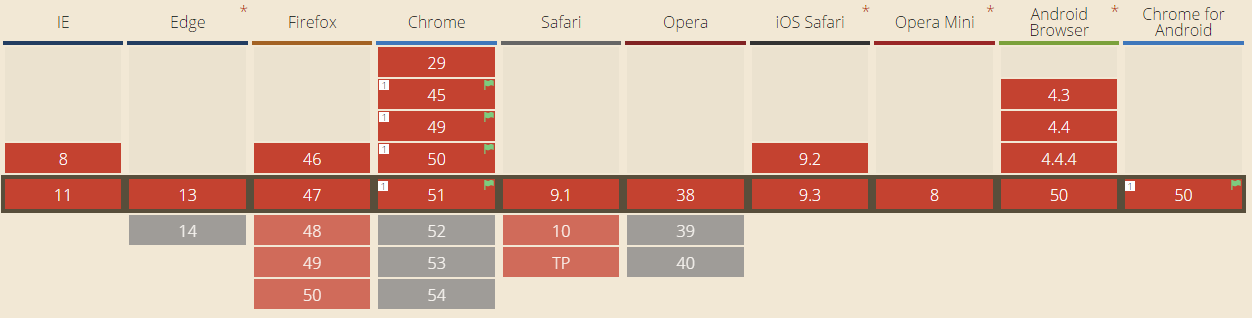
\includegraphics[width=10cm,frame]{caniuse_bluetooth}
	\caption{Support de l'API Web Bluetooth par les différents navigateurs.}
	\label{caniuse-bluetooth}
\end{figure}

\subsection{Accéléromètre et Gyroscope}
L'approche par accéléromètre et gyroscope est différente, car elle implique d'utiliser les capteurs internes du smartphone pour calculer une position. HTML5 fournit une API pour détecter l'orientation et les déplacements du dispositif. Autrement dit, l'accès à l'accéléromètre et au gyroscope est possible depuis un navigateur Internet.

A l'aide de l'accélération, il est théoriquement possible de calculer une position. Cependant, les valeurs de ces capteurs comportent un bruit et, pour calculer une position, il faut double-intégrer l'accélération. Cela implique qu'il faut double-intégrer le bruit et cela va créer un \textit{drift}. En quelques secondes, l'erreur peut s'élever à une vingtaine de centimètres. En outre, le gyroscope peut avoir une valeur erronée, due à la suppression de la gravité. En d'autres termes, une erreur d'un degré sur la valeur du gyroscope représente plusieurs mètres d'erreur en quelques secondes \cite{google-SensorFusion}. 

Le but de cette approche était fondamentalement d'estimer la position de l'utilisateur, sans pour autant connaître la valeur exacte. Les démarches et réflexions prouvent qu'une approximation n'est pas envisageable avec ces capteurs.